% !TEX root = ../../main.tex

\chapter{Evaluation}
\label{chapter:evaluation-discussion}
This chapter shows Contribution \textbf{C.2}: A robust cost estimator for Amalur's factorized ML framework, and a comparison with the SOTA in \autoref{sec:eval-model-evaluation}. Before that, we show how results were collected in \autoref{sec:6experiment-setup}. The \hyperref[sec:eval-discussion]{third section} of this chapter provides an in-depth interpretation of the results as well as a critical view on the implications and limitations of this work.

\section{Experiment Setup}
\label{sec:6experiment-setup}

This section goes into detail about anything needed to replicate the results. This includes the experimental environment (\hyperref[subsec:6-software]{Software}, \hyperref[subsec:6-datasets]{Datasets} \& \hyperref[subsec:6-hardware]{Hardware}),  and how the data was treated to ensure sound results for the cost estimators (\hyperref[subsec:6-validation-strategy]{validation strategy}). For further details and implementations please refer to the GitHub repository\footnote{\todo{TODO}}.

\subsection{Software}
\label{subsec:6-software}
The factorized ML framework (Amalur \cite{amalur}) is implemented in Python (3.10.4) and uses SciPy (1.8.0), NumPy (1.22.4) and CuPy (12.1.1). All experiments where ran in a Docker container with an image based on Nvidia's base image with CUDA 12.1.1 and Ubuntu 20.04\footnote{\href{https://hub.docker.com/layers/nvidia/cuda/12.1.1-devel-ubuntu20.04/images/sha256-5bd13c67a4479a1c13238b470d89a92937ce68ba5f21b930d50c463e3314f657?context=explore}{nvidia/cuda:12.1.1-devel-ubuntu20.04}}.

The choice to use CuPy as the backend for the factorized ML framework was made to ensure that the experiments could be run on both CPU and GPU. CuPy is a GPU-accelerated library for numerical computations that is compatible with NumPy and SciPy \cite{cupy_learningsys2017}. This allows for minimal changes to the codebase whether you are using GPU or CPU. To allow for exploitation of multiple cores for sparse matrix multiplication\footnote{\url{https://github.com/flatironinstitute/sparse_dot}} we use MKL (Intel Math Kernel Library) \cite{intel-mkl} as NumPy's backend for the CPU experiments.

For collecting the GPU metrics we use NVIDIA's Nsight Compute (ncu)\footnote{\url{https://docs.nvidia.com/nsight-compute/NsightComputeCli/index.html}} which is a command-line profiler that collects detailed performance metrics from the GPU. The metrics are collected in a CSV file for downstream analysis, detailed in \autoref{sec:5-feature-engineering}. The cost estimators were created with Scikit-learn \cite{scikit-learn}.

\subsection{Datasets}
\label{subsec:6-datasets}
The datasets used in the experiments are a mix of synthetic and real-world datasets. The synthetic datasets are used to generate a training set to train the cost estimators on. The real-world datasets are used to validate the cost estimators on unseen data.

\subsubsection{Synthetic Datasets}
To create the synthetic datasets with a wide variety of data characteristics the data generator from \cite{schijndel_cost_estimation} was used, which in turn is an adaptation of the data generator\footnote{\url{https://github.com/delftdata/valentine-data-fabricator}} from \cite{valentine-data-generator}.

In total, we generated $2415$ datasets, each being a two-table join. All other parameters were varied, the values are shown in \autoref{tab:6-synthetic-dataset-characteristics}.

\todo{Expand this! Explain star schema (and show example)?}

\begin{table}[ht]
  \centering
  \begin{tabular}{llr}
    \toprule
    Data Characteristic             & Symbol    & Range                              \\ \midrule \midrule
    Target Sparsity                 & $e_T$     & $[ 0.0\text{,\ \ } 0.9]$           \\
    $S_1$ (Entity) table rows       & $r_{S_1}$ & $[ 40,000\text{,\ \ } 1,000,000]$  \\
    $S_1$ (Attribute) table rows    & $r_{S_2}$ & $[ 526\text{,\ \ } 1,000,000]$     \\
    $S_1$ (Entity) table columns    & $c_{S_1}$ & $[ 1\text{,\ \ } 50]$              \\
    $S_1$ (Attribute) table columns & $c_{S_2}$ & $[ 2\text{,\ \ } 50]$              \\
    Target table rows               & $r_T$     & $[ 60,000 \text{,\ \ } 1,000,000]$ \\
    Target table columns            & $c_T$     & $[ 11\text{,\ \ } 100]$            \\
    Tuple ratio                     & $\rho$    & $[ 1\text{,\ \ } 190]$             \\
    Feature ratio                   & $\tau$    & $[ 0.2\text{,\ \ } 1]$             \\
    Join Type                       & $j_T$     & Inner, left or outer.              \\
    Selectivity                     & $\sigma$  & $[ 1.0\text{,\ \ } 2.0]$           \\
    \bottomrule
  \end{tabular}
  \caption{Ranges of data characteristics for the generated synthetic datasets}
  \label{tab:6-synthetic-dataset-characteristics}
\end{table}


\subsubsection{Real-world Datasets}
The synthetic datasets are convenient for testing and training purposes. However, to assess whether the cost estimators are generalizable to real-world data, we use real-world datasets for validation.

\paragraph{Project Hamlet \cite{2016-hamlet-sigmod}}
The Hamlet datasets are widely used in related literature \cite{2016-hamlet-sigmod, amalur, morpheus,orion_learning_gen_lin_models}. The Hamlet datasets are a set 7 datasets specifically designed to mimic data integration scenarios is an ML workflow. The original datasets where created to evaluate inner join scenario's. As we are also interested in other join types, some rows were removed from different source tables for these join types. The data characteristics of these datasets are shown in \autoref{tab:6-hamlet-characteristics}.


\begin{table}[ht]
  \centering
  \begin{tabular}{p{0.12\linewidth}rrrrrrr}
    \toprule
    Dataset$\rightarrow$ Characteristic $\downarrow$ & Book  & Expedia & Flight & Lastfm & Movie & Walmart & Yelp  \\
    \midrule \midrule
    $r_T$                                            & 253K  & 942K    & 66.5K  & 344K   & 1M    & 422K    & 216K  \\
    $c_T$                                            & 81.7K & 52.3K   & 13.7K  & 55.3K  & 13.3K & 2.44K   & 55.6K \\
    $n$                                              & 2     & 3       & 4      & 2      & 2     & 3       & 2     \\
    $r_{S_1}$                                        & 27.9K & 942K    & 66.5K  & 5K     & 6.04K & 422K    & 11.5K \\
    $r_{S_2}$                                        & 50K   & 11.9K   & 540    & 50K    & 3.71K & 2.34K   & 43.9K \\
    $r_{S_3}$                                        &       & 37K     & 3.17K  &        &       & 45      &       \\
    $r_{S_4}$                                        &       &         & 3.17K  &        &       &         &       \\
    $c_{S_1}$                                        & 28K   & 27      & 20     & 5.02K  & 9.51K & 1       & 11.7K \\
    $c_{S_2}$                                        & 53.6K & 12K     & 718    & 50.2K  & 3.84K & 2.39K   & 43.9K \\
    $c_{S_3}$                                        &       & 40.2K   & 6.46K  &        &       & 53      &       \\
    $c_{S_4}$                                        &       &         & 6.47K  &        &       &         &       \\
    \bottomrule
  \end{tabular}
  \caption[Hamlet dataset characteristics]{Hamlet dataset characteristics. $r$ is the number of rows, $c$ is the number of columns, and $n$ is the number of tables. The subscripts denote which table the characteristic belongs to. }
  \label{tab:6-hamlet-characteristics}
\end{table}


\paragraph{TPCx-AI \cite{tpcx-ai}} We also evaluate on a scenario even more realistic than Hamlet, as it is based on a real-world benchmark used to evaluate end-to-end ML platforms. As that is not the focus of this work, we use only two out of the ten use cases, namely the first and the tenth use case. This benchmark also provides a data generator with scalable generation capabilities, through setting different scale factors from $0.01-0.5$ we generated $18$ datasets for each use case. The data characteristics of the resulting datasets can be found in \autoref{fig:tpcx-ai-data-chars}.
\begin{figure}
  \centering
  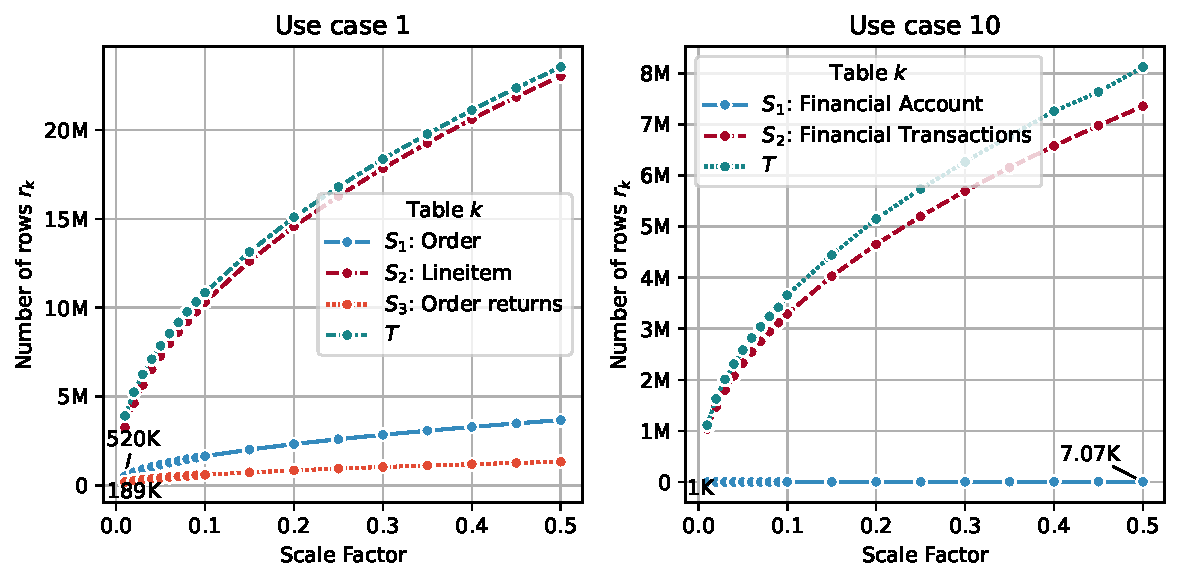
\includegraphics[width=\linewidth]{chapters/06_evaluation/figures/tpcx-ai-data-chars.pdf}
  \caption[TPCx-AI dataset sizes for used scale factors.]{TPCx-AI dataset sizes for used scale factors. The number of columns is independent of the scale factors. For use case 1: $c_1=3, c_2=4, c_3=3, c_T=7$. For use case 10: $c_1=2, c_2=7, c_T=5$.}
  \label{fig:tpcx-ai-data-chars}
\end{figure}

The first use case is a join between three tables. First the lineitem table is joined with the order returns data which, in turn, is joined with the orders table. This results in a table with $c_T=7$ columns and a row for each product sold in an order. In the TPCx-AI benchmark customer segmentation is done using KMeans clustering on this dataset. We instead test all four ML models discussed in this thesis as we are not necessarily interested in the utility of the final classifier, but we are interested in the training process. The second use case is a join between two tables. The transaction table is joined with the customer table, resulting in a table with $c_T=5$ columns which can be used to detect fraudulent transactions. We use the same models as in the first use case. The complete dataset schema detailing the involved tables and columns can be found in \autoref{fig:appendix-tpc-ai-schema}.



\subsection{Hardware}
\label{subsec:6-hardware}

The experiments are run on a relatively large set of different machines because of the need to test on varying hardware. Most experiments were run on the Delft AI Cluster\footnote{\url{https://daic.tudelft.nl/}}, which made it possible to run experiments on different GPU architectures. Because profiling was not possible on this cluster, some profiling experiments were run on a local machine, AWS, and resources of the Web Information Systems group\footnote{\url{https://www.wis.ewi.tudelft.nl/}}. The exact overview of which experiment was run on which machines is shown in \autoref{tab:6-hardware-overview}.

\begin{table}[ht]
  \centering
  % LTeX: enabled=false
\begin{tabular}{p{0.15\linewidth}p{0.19\linewidth}p{0.10\linewidth}p{0.20\linewidth}l}
    \toprule
    Experiment type                                                 & Machine                                                         & \hspace{0pt}Architecture                                  & Compute Unit           & Experiment       \\
    \midrule\midrule
    \multirow[t]{3}{*}{\parbox{1\linewidth}{\vspace{1.5cm}profile}} & WIS ST4                                                         & Ampere                                                    & GPU A40                & \texttt{GPU-P-1} \\
    \cline{2-5}
                                                                    & AWS G5.xlarge                                                   & Ampere                                                    & GPU A10G               & \texttt{GPU-P-2} \\
    \cline{2-5}
                                                                    & Personal Workstation                                            & Turing                                                    & GPU 1660Ti             & \texttt{GPU-P-3} \\
    \cline{1-5}
    \multirow[t]{8}{*}{\parbox{1\linewidth}{\vspace{4cm}runtime}}   & \multirow[t]{5}{*}{\parbox{1\linewidth}{\vspace{2cm}DAIC}}      & Ampere                                                    & GPU A40                & \texttt{GPU-T-1} \\

                                                                    &                                                                 & Volta                                                     & GPU V100               & \texttt{GPU-T-2} \\

                                                                    &                                                                 & Pascal                                                    & GPU P100               & \texttt{GPU-T-3} \\

                                                                    &                                                                 & Turing                                                    & GPU 2080Ti             & \texttt{GPU-T-4} \\

                                                                    &                                                                 & Pascal                                                    & GPU 1080Ti             & \texttt{GPU-T-5} \\
    \cline{2-5}
                                                                    & \multirow[t]{3}{*}{\parbox{1\linewidth}{\vspace{2.3cm}WIS ST4}} & \multirow[t]{3}{*}{\parbox{1\linewidth}{\vspace{2.3cm}—}} & EPYC 7H12 CPU 8 cores  & \texttt{CPU-T-1} \\

                                                                    &                                                                 &                                                           & EPYC 7H12 CPU 16 cores & \texttt{CPU-T-2} \\

                                                                    &                                                                 &                                                           & EPYC 7H12 CPU 32 cores & \texttt{CPU-T-3} \\
    \cline{1-5}
    \bottomrule
\end{tabular}

  \caption[Experiment to machine mapping]{Experiment to machine mapping. The experiment type is either profiling or runtime. Profiling experiments are used to collect the hardware specific metrics for our training data. Runtime experiments are used to gather data on the runtime of the factorized ML framework compared to materialized learning.}
  \label{tab:6-hardware-overview}
\end{table}

\subsection{Experiment Setting}
To ensure reliable training data all runtime experiments were run with a repetition count of $30$. The profiling experiments were not repeated, as NCU ensures actionable and deterministic results through, e.g., replaying kernel launches \cite{nsight_compute}. All experiments were run in a containerized environment to ensure reproducibility. The profiling experiments were run with the same image as the runtime experiments, to ensure that the same environment was used for both. Docker\footnote{\url{https://www.docker.com/}} was used as the container runtime, except on the DAIC cluster which enforces the use of Apptainer\footnote{\url{https://apptainer.org/}} image.

\subsection{Validation Strategy}
\label{subsec:6-validation-strategy}

As the possible set of data, model, and hardware characteristics is extremely large, we need to be confident in the ability of our estimator to make accurate predictions for unseen scenarios. To ensure this we use a very strict train-validate-test split. 70\% of the samples from the synthetic datasets are used in the training set. The remaining 30\% is used as a validation set. The real-world datasets are used solely as a test set. As they are not used in the training of the cost estimators they should give an accurate view of the performance in unseen scenarios, whether this is actually the case is shown in \autoref{subsec:6-generalizability}. To guarantee the same robustness in the hardware dimension we use a similar approach, completely keeping the samples of \texttt{GPU-T-5} separate for testing. For the last dimension, the model characteristics, we carry out an ablation study (see \autoref{subsubsec:6-ablation}) to see the effect of leaving out different models on the performance of the cost estimators.


% \begin{figure}[ht]
%   \centering
%   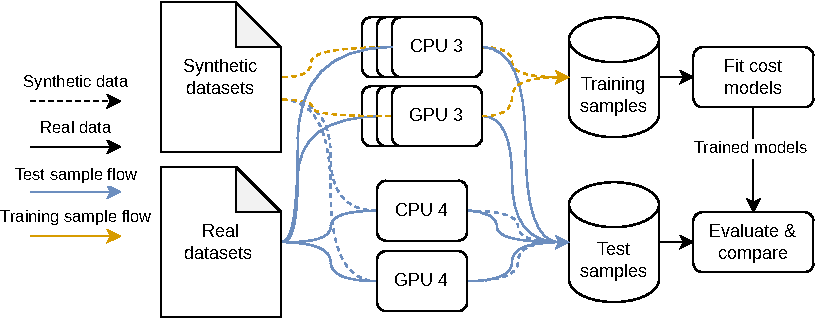
\includegraphics[width=0.8\linewidth]{chapters/06_evaluation/figures/experiment-pipeline.pdf}
%   \caption{\todo{update} Overview of the planned experiments: combinations of datasets and machines we run the experiments
%     on. }
%   \label{fig:enter-label}
% \end{figure}

\section{Cost Model Performance and Comparative Analysis}
\label{sec:eval-model-evaluation}

In this section we answer
\begin{itemize}
  \item[RQ.2] How can we accurately predict the optimal choice between factorized or materialized training of a Machine Learning model, on CPU and GPU, through leveraging knowledge about model, data, and hardware characteristics?
\end{itemize}

We first display that the cost estimator generalizes well to new scenarios. Then we show how the cost estimators compare to the SOTA in cost estimation for Factorized ML training.

\subsection{Exploring Generalizability}
\label{subsec:6-generalizability}
The goal of this thesis is to create a cost estimator that can accurately predict the optimal choice between factorized and materialized training of a Machine Learning model. To ensure that this cost estimator also performs well in unseen scenarios, i.e., it is not overfitting to the training data, we evaluate the cost estimators on the real-world datasets, and on new hardware. The results are shown in \autoref{fig:6-generalization}.

\begin{figure}
  \centering
  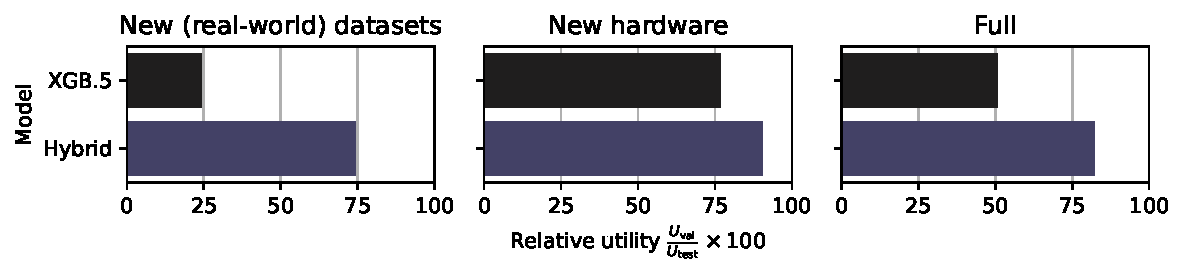
\includegraphics[width=\linewidth]{chapters/06_evaluation/figures/eval_generalization.pdf}
  \caption{Evaluation and comparison of cost model's relative performance on new scenarios. The y-axis shows the relative performance, defined as total time saved, with regard to the validation set, for each group of scenario types. A value of 100\% means that the cost estimator performs equally well on the validation set as on the training set, when measured by $\frac{\text{time saved}}{\text{max. possible time saved}}$.}
  \label{fig:6-generalization}
\end{figure}

The \hyperref[fig:6-generalization]{figure} shows that there are large differences for how well the cost estimators generalize to new scenarios. The analytical models show the best relative performance which can be explained by the fact they are not prone to overfitting, and already do not perform very well on the training set. The statistical models show okay relative performance on the real datasets but very poor performance on the new hardware meaning they did not capture the relation between hardware characteristics and cost well. The XGBoost models show great relative performance on new hardware, but poor performance on the real datasets. The hybrid model combines the strong points of the XGBoost and statistical models, showing good relative performance of 82\% on the full dataset.

\subsubsection{Ablation Study}
\label{subsubsec:6-ablation}
\todo{Show the effect of including/excluding models on the performance of the cost estimators.}

\subsection{Cost Estimator Comparison}
\label{subsec:6-sota-comparison}

In this section, we compare the performance of our cost models to the SOTA cost estimators. The comparison is based on the same test set used in the previous sections, which includes real datasets and new hardware configurations.

\autoref{fig:6-sota-comparison} presents the results of this comparison. The left plot shows the precision, accuracy, f1 score and recall score of the cost estimators. The right plot shows the total time saved by the cost estimators for the set of scenarios.

From the figure we can infer how each estimator behaves with regard to the precision/recall trade-off. The SOTA cost estimators show poor precision, but higher recall. This means that they are more lenient towards predicting a positive label, which in this case means that the factorized training is faster. MorpheusFI \cite{MorpheusFI} shows the best recall, but that is explained when looking at the accuracy and precision. It just labels all cases as positive, resulting in a total time loss of $13,000$ seconds. Morpheus \cite{orion_learning_gen_lin_models} shows a total time loss of around $7000$ seconds as it is slightly more conservative than MorpheusFI. Amalur \cite{amalur} shows a total time loss of around $500$ seconds, which shows it is a better estimator than Morpheus and MorpheusFI. The Hybrid cost estimators proposed in this thesis shows a total time saved of around $1350$ seconds, with an accuracy of $95\%$, which is a significant improvement over the SOTA.

\begin{figure}[ht]
  \centering
  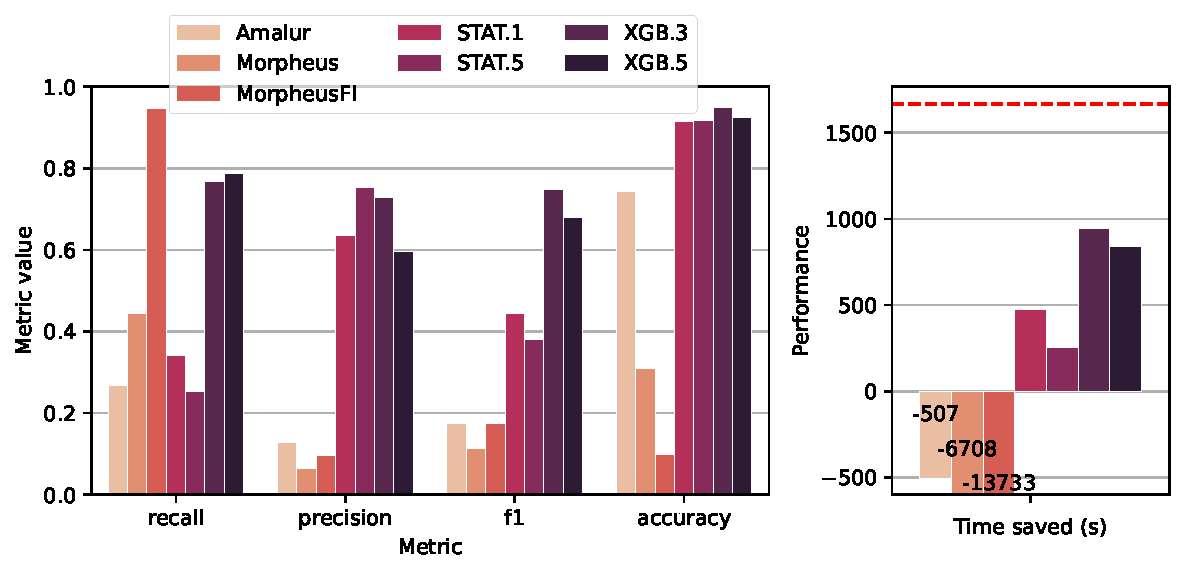
\includegraphics[width=\linewidth]{chapters/06_evaluation/figures/eval_sota_results.pdf}
  \caption{Comparison of the cost estimators. Performance evaluated on the test set (real datasets and new hardware).}
  \label{fig:6-sota-comparison}
\end{figure}

\section{Discussion}
\label{sec:eval-discussion}
We have shown our Hybrid cost estimator is capable of accurately predicting the optimal choice between factorized and materialized training of a Machine Learning model, on both CPU and GPU. The hybrid estimator shows good generalizability to new scenarios, and outperforms the SOTA in cost estimation for Factorized ML training. However, there are some limitations to this work.

The first important note is that the SOTA cost estimators were not created with training on GPUs in mind. This is a significant limitation. We have shown that the trade-off between factorization and materialization behaves drastically different between CPU and GPU training.

The second limitation is that the cost estimators were trained on synthetic data. This is a common practice in cost estimation for ML training, but it is not ideal. The synthetic datasets were created to mimic real-world data, but there are always differences. We have shown that the cost estimators generalize well to real-world data, but there is always a risk that the cost estimators are overfitting to the synthetic data, and the good performance on Hamlet and TPCx-AI is a coincidence. This limitation also applies to the hardware dimension. We have shown that the cost estimators generalize well to new hardware, but there is always a risk that the new hardware settings are not representative enough of hardware settings in real world applications.

Despite these limitations, we believe that our work provides a valuable contribution to the field of cost estimation for ML training. Our hybrid cost estimator shows promising results and outperforms the SOTA in many scenarios. We hope that our work will inspire further research in this area.

\section{Conclusion}
\label{sec:eval-conclusion}

In this chapter, we have presented the evaluation of our hybrid cost estimator for factorized and materialized ML training. We have shown that our estimator is capable of accurately predicting the optimal choice between factorized and materialized training, and that it outperforms the SOTA in cost estimation.

In the next chapter, we will discuss the future work and potential improvements that can be made to our cost estimator.
